% FORMA User Manual
% FFT-based Orbit Response Matrix Analyzer
% =============================================================================
\documentclass[11pt,a4paper,twoside]{report}

% ── Geometry ──────────────────────────────────────────────────────────────────
\usepackage[
  top=2.5cm, bottom=2.5cm, inner=2.8cm, outer=2.2cm,
  headheight=14pt, marginparwidth=1.6cm
]{geometry}

% ── Fonts & Encoding ─────────────────────────────────────────────────────────
\usepackage[T1]{fontenc}
\usepackage[utf8]{inputenc}
\usepackage{lmodern}
\usepackage{microtype}

% ── Colour Palette (mirrors the app) ─────────────────────────────────────────
\usepackage[dvipsnames,svgnames,x11names]{xcolor}
\definecolor{bgdark}{HTML}{0f172a}
\definecolor{surface}{HTML}{1e293b}
\definecolor{card}{HTML}{16213c}
\definecolor{accent}{HTML}{38bdf8}
\definecolor{accent2}{HTML}{34d399}
\definecolor{warncol}{HTML}{f97316}
\definecolor{dangercol}{HTML}{ef4444}
\definecolor{mutedtext}{HTML}{94a3b8}
\definecolor{chapblue}{HTML}{1d4ed8}
\definecolor{secblue}{HTML}{2563eb}
\definecolor{lightbg}{HTML}{f0f4ff}
\definecolor{codebg}{HTML}{f1f5f9}

% ── Maths ─────────────────────────────────────────────────────────────────────
\usepackage{amsmath,amssymb,mathtools,bm}

% ── Graphics & Figures ────────────────────────────────────────────────────────
\usepackage{graphicx,float}
\usepackage{tikz}
\usetikzlibrary{
  shapes.geometric, arrows.meta, positioning, calc,
  backgrounds, fit, shadows, decorations.markings
}

% ── Tables ────────────────────────────────────────────────────────────────────
\usepackage{booktabs,tabularx,array,colortbl,multirow,longtable}

% ── Boxes & Callouts ─────────────────────────────────────────────────────────
\usepackage[most]{tcolorbox}
\tcbuselibrary{skins,breakable}

\newtcolorbox{notebox}[1][]{
  enhanced, breakable,
  colback=accent!5, colframe=accent!70!black,
  fonttitle=\bfseries, title={#1},
  left=4pt, right=4pt, top=4pt, bottom=4pt,
  boxrule=0.8pt, arc=2pt,
  before upper={\parindent0pt},
}

\newtcolorbox{warnbox}[1][]{
  enhanced, breakable,
  colback=warncol!6, colframe=warncol!80!black,
  fonttitle=\bfseries, title={#1},
  left=4pt, right=4pt, top=4pt, bottom=4pt,
  boxrule=0.8pt, arc=2pt,
  before upper={\parindent0pt},
}

\newtcolorbox{dangerbox}[1][]{
  enhanced, breakable,
  colback=dangercol!6, colframe=dangercol!80!black,
  fonttitle=\bfseries, title={#1},
  left=4pt, right=4pt, top=4pt, bottom=4pt,
  boxrule=0.8pt, arc=2pt,
  before upper={\parindent0pt},
}

\newtcolorbox{defbox}[1][]{
  enhanced, breakable,
  colback=lightbg, colframe=chapblue!60,
  fonttitle=\bfseries\color{chapblue}, title={#1},
  left=4pt, right=4pt, top=4pt, bottom=4pt,
  boxrule=0.8pt, arc=2pt,
  before upper={\parindent0pt},
}

\newtcolorbox{stepbox}[1][]{
  enhanced, breakable,
  colback=accent2!4, colframe=accent2!70!black,
  fonttitle=\bfseries, title={#1},
  left=4pt, right=4pt, top=4pt, bottom=4pt,
  boxrule=0.8pt, arc=2pt,
  before upper={\parindent0pt},
}

% ── Code Listings ─────────────────────────────────────────────────────────────
\usepackage{listings}
\lstset{
  basicstyle=\ttfamily\small,
  backgroundcolor=\color{codebg},
  frame=single, rulecolor=\color{mutedtext!40},
  breaklines=true, breakatwhitespace=true,
  columns=fullflexible, keepspaces=true,
  showstringspaces=false,
  keywordstyle=\color{chapblue}\bfseries,
  commentstyle=\color{mutedtext}\itshape,
  stringstyle=\color{accent2!80!black},
  xleftmargin=4pt, xrightmargin=4pt,
  aboveskip=6pt, belowskip=6pt,
}

% ── Headers & Footers ────────────────────────────────────────────────────────
\usepackage{fancyhdr}
\pagestyle{fancy}
\fancyhf{}
\fancyhead[LE]{\small\textcolor{mutedtext}{\leftmark}}
\fancyhead[RO]{\small\textcolor{mutedtext}{\rightmark}}
\fancyfoot[C]{\small\textcolor{mutedtext}{\thepage}}
\renewcommand{\headrulewidth}{0.4pt}
\renewcommand{\footrulewidth}{0pt}

% ── Chapter & Section Formatting ─────────────────────────────────────────────
\usepackage{titlesec}

\titleformat{\chapter}[display]
  {\normalfont\huge\bfseries\color{chapblue}}
  {\chaptertitlename\ \thechapter}{16pt}{\Huge}
\titlespacing*{\chapter}{0pt}{-20pt}{30pt}

\titleformat{\section}
  {\normalfont\Large\bfseries\color{secblue}}
  {\thesection}{1em}{}
\titleformat{\subsection}
  {\normalfont\large\bfseries\color{secblue!80!black}}
  {\thesubsection}{1em}{}
\titleformat{\subsubsection}
  {\normalfont\normalsize\bfseries\color{secblue!60!black}}
  {\thesubsubsection}{1em}{}

% ── Hyperlinks ────────────────────────────────────────────────────────────────
\usepackage[
  colorlinks=true, linkcolor=chapblue, urlcolor=accent!70!black,
  citecolor=accent2!70!black, bookmarks=true,
  pdfauthor={FORMA Development Team},
  pdftitle={FORMA User Manual},
  pdfsubject={FFT-based Orbit Response Matrix Analyzer},
]{hyperref}
\usepackage{bookmark}

% ── Enumeration ───────────────────────────────────────────────────────────────
\usepackage{enumitem}
\setlist[itemize]{leftmargin=*, itemsep=2pt, parsep=1pt}
\setlist[enumerate]{leftmargin=*, itemsep=2pt, parsep=1pt}

% ── Misc ──────────────────────────────────────────────────────────────────────
\usepackage{parskip}
\setlength{\parskip}{6pt plus 1pt minus 1pt}
\setlength{\parindent}{0pt}

\newcommand{\forma}{\textsc{Forma}}
\newcommand{\acnet}{\textsc{Acnet}}
\newcommand{\menupath}[1]{\texttt{\small #1}}
\newcommand{\btn}[1]{\colorbox{accent!12}{\texttt{\small #1}}}
\newcommand{\kbd}[1]{\colorbox{surface!20}{\texttt{\small #1}}}
\newcommand{\field}[1]{\textit{#1}}

% ═════════════════════════════════════════════════════════════════════════════
\begin{document}

% ── Title Page ────────────────────────────────────────────────────────────────
\begin{titlepage}
\begin{tikzpicture}[remember picture, overlay]
  % Background
  \fill[bgdark] (current page.south west) rectangle (current page.north east);
  % Accent bar
  \fill[accent] ([yshift=-6cm]current page.north west)
    rectangle ([yshift=-6.15cm]current page.north east);
  % Decorative arc
  \fill[accent!15] ([yshift=-8cm, xshift=-3cm]current page.north east)
    circle [x radius=8cm, y radius=4cm];
\end{tikzpicture}

\vspace*{3cm}
\begin{center}
  {\fontsize{52}{60}\selectfont\bfseries\textcolor{white}{FORMA}}\\[12pt]
  {\Large\textcolor{accent}{FFT-based Orbit Response Matrix Analyzer}}\\[30pt]
  \textcolor{mutedtext}{\rule{8cm}{0.5pt}}\\[20pt]
  {\large\textcolor{white}{User Manual}}\\[6pt]
  {\normalsize\textcolor{mutedtext}{Version 1.0 --- \today}}\\[60pt]
  {\normalsize\textcolor{mutedtext}{Fermilab Accelerator Division}}\\[4pt]
  {\small\textcolor{mutedtext}{High-Level Application Suite}}
\end{center}
\end{titlepage}

% ── Front Matter ──────────────────────────────────────────────────────────────
\pagenumbering{roman}

\tableofcontents
\clearpage
\listoffigures
\clearpage

% ═════════════════════════════════════════════════════════════════════════════
\pagenumbering{arabic}

% ═════════════════════════════════════════════════════════════════════════════
\chapter{Introduction}
% ═════════════════════════════════════════════════════════════════════════════

\section{What is FORMA?}

\forma{} (\textbf{F}FT-based \textbf{O}rbit \textbf{R}esponse \textbf{M}atrix \textbf{A}nalyzer) is a high-level application for measuring and analysing the \emph{orbit response matrix} (ORM) of a circular particle accelerator. It drives corrector magnets with sinusoidal excitations, records beam-position monitor (BPM) readings, and extracts the linear transfer function between each corrector--BPM pair using spectral (FFT) analysis.

\begin{defbox}[Orbit Response Matrix]
The orbit response matrix $\mathbf{R}$ relates small changes in corrector strengths $\Delta\theta_j$ to the resulting changes in closed-orbit position $\Delta x_i$ at each BPM:
\[
  \Delta x_i \;=\; \sum_{j} R_{ij}\,\Delta\theta_j
  \qquad\Longleftrightarrow\qquad
  \Delta\mathbf{x} = \mathbf{R}\,\Delta\boldsymbol{\theta}
\]
Each element $R_{ij}$ has units of \emph{position per kick} (e.g.\ mm\,/\,A or mm\,/\,mrad).
\end{defbox}

\section{Key Capabilities}

\begin{itemize}
  \item \textbf{AC excitation scans} --- sinusoidal modulation of correctors, either simultaneously (fast) or sequentially (robust).
  \item \textbf{FFT-based extraction} --- spectral isolation of the drive response from broadband noise.
  \item \textbf{Error estimation} --- rigorous propagation of spectral noise into per-element uncertainties.
  \item \textbf{Safety monitoring} --- real-time watchdog that aborts scans if orbit deviations exceed configurable thresholds.
  \item \textbf{Integrated analysis} --- built-in heatmap display, plus an advanced viewer with SVD-based beta-function estimation, cosine-similarity analysis, and interactive slice plots with error bars.
\end{itemize}

\section{Physics Background}\label{sec:physics}

In a circular accelerator the transverse closed orbit at location~$s_i$ satisfies
\begin{equation}\label{eq:orm-theory}
  R_{ij}
  \;=\;
  \frac{\sqrt{\beta_i\,\beta_j}}{2\sin(\pi Q)}\,
  \cos\!\bigl(\lvert\psi_i - \psi_j\rvert - \pi Q\bigr),
\end{equation}
where $\beta_i,\beta_j$ are the Courant--Snyder betatron functions at the BPM and corrector, $Q$ is the betatron tune, and $\psi$ is the betatron phase advance. Measuring $\mathbf{R}$ therefore gives direct access to the optics of the machine.

\subsection{Why AC Excitation?}

A DC bump measurement (apply a static kick, measure the orbit change) is sensitive to any drift that occurs between the ``bump-on'' and ``bump-off'' readings. \forma{} instead modulates each corrector at a known frequency and extracts only the coherent response at that frequency via the FFT. This rejects:

\begin{itemize}
  \item slow drifts (appear at DC, which is excluded),
  \item 50/60\,Hz mains ripple (appears at different frequencies),
  \item broadband BPM noise (spread across all bins, diluted by $\sqrt{N}$).
\end{itemize}

The result is a cleaner, higher-SNR measurement of $R_{ij}$, especially in a noisy operational environment.


% ═════════════════════════════════════════════════════════════════════════════
\chapter{Mathematical Algorithms}\label{ch:math}
% ═════════════════════════════════════════════════════════════════════════════

This chapter gives a self-contained derivation of every formula used in \forma{}.

% ─────────────────────────────────────────────────────────────────────────────
\section{Discrete Fourier Transform}\label{sec:dft}

Given a real-valued time series $x[n]$, $n=0,\dots,N{-}1$, sampled at interval $\Delta t$, the DFT is
\begin{equation}\label{eq:dft}
  X[k] = \sum_{n=0}^{N-1} x[n]\,e^{-j2\pi kn/N},
  \qquad k=0,\dots,N{-}1.
\end{equation}
The corresponding frequency of bin~$k$ is
\begin{equation}\label{eq:freq}
  f_k = \frac{k}{N\,\Delta t}, \qquad k=0,\dots,\lfloor N/2\rfloor - 1.
\end{equation}

\subsection{One-Sided Amplitude Spectrum}

For a real signal, $X[k]$ and $X[N{-}k]$ are conjugate pairs. The one-sided amplitude spectrum (positive frequencies only) is defined as:
\begin{equation}\label{eq:amp}
  A[k] = \frac{2}{N}\,\lvert X[k]\rvert,
  \qquad k=1,\dots,\lfloor N/2\rfloor - 1.
\end{equation}
The factor $2/N$ ensures that for a pure sinusoid $x[n]=A_0\sin(2\pi f_0 n\,\Delta t)$, the peak amplitude $A[k_0]$ recovers the physical amplitude~$A_0$, independent of~$N$.

\begin{notebox}[DC Component]
The DC bin ($k{=}0$) is always excluded from analysis. Before computing the FFT the mean is subtracted from the signal: $s[n] = x[n] - \bar{x}$.
\end{notebox}

% ─────────────────────────────────────────────────────────────────────────────
\section{Drive Frequency Detection}\label{sec:freqdetect}

For each corrector, \forma{} finds the dominant excitation frequency by:
\begin{enumerate}
  \item Computing the one-sided amplitude spectrum $A_c[k]$ (Eq.~\ref{eq:amp}).
  \item Setting $A_c[0]=0$ (ignore DC).
  \item Selecting the bin with the largest amplitude:
    \begin{equation}\label{eq:peakbin}
      k^{*} = \arg\max_{k\ge1} A_c[k].
    \end{equation}
  \item Recording the drive frequency $f_c = k^{*}/(N\,\Delta t)$ and the complex Fourier coefficient
    \begin{equation}
      \tilde{A}_c = \frac{2}{N}\,X_c[k^{*}].
    \end{equation}
\end{enumerate}

% ─────────────────────────────────────────────────────────────────────────────
\section{Transfer Function and Response Matrix}\label{sec:transfer}

For each (BPM~$i$, corrector~$j$) pair, \forma{} computes the complex transfer function at the corrector's drive frequency:
\begin{equation}\label{eq:transfer}
  H_{ij}
  = \frac{\tilde{A}_{b,i}[k^{*}_j]}{\tilde{A}_{c,j}[k^{*}_j]}
  = \frac{(2/N)\,X_{b,i}[k^{*}_j]}{(2/N)\,X_{c,j}[k^{*}_j]}\,,
\end{equation}
where subscripts $b$ and $c$ denote BPM and corrector respectively. The $2/N$ factors cancel, but are retained for clarity. The response matrix element is the \emph{real part} of this transfer function:
\begin{equation}\label{eq:Rij}
  \boxed{\;R_{ij} = \operatorname{Re}(H_{ij}) = \lvert H_{ij}\rvert\cos\phi_{ij}\;}
\end{equation}
where $\phi_{ij}$ is the phase of the transfer function.

\begin{notebox}[Why take the real part?]
For a quasi-static corrector kick (excitation frequency $\ll$ betatron frequency), the orbit response is in phase with the drive ($\phi\approx0$ or $\pi$). Taking $\operatorname{Re}(H)$ preserves the \emph{sign} of the response (positive = same direction as kick, negative = opposite), which is essential for orbit correction algorithms. The imaginary part, representing any phase lag, is discarded.
\end{notebox}

% ─────────────────────────────────────────────────────────────────────────────
\section{Noise Estimation}\label{sec:noise}

Accurate error bars require estimating the spectral noise floor of both the corrector and the BPM signals, excluding the deliberate drive signal.

\subsection{Corrector Noise $\sigma_c$}

After computing the corrector's amplitude spectrum, \forma{} zeros out the drive peak and its two nearest neighbours on each side (a $\pm2$ bin exclusion zone):
\begin{equation}
  \mathcal{E}_c = \{k^{*}{-}2,\;\dots,\;k^{*}{+}2\},
\end{equation}
then computes the RMS of the remaining bins:
\begin{equation}\label{eq:corrnoise}
  \sigma_c = \sqrt{\frac{1}{N_{\text{bins}}}
    \sum_{k\notin\mathcal{E}_c,\,k\ge1} \bigl\lvert A_c[k]\bigr\rvert^2}\,.
\end{equation}

\subsection{BPM Noise $\sigma_b$}

BPM spectra contain peaks at \emph{every} corrector's drive frequency (because all correctors affect all BPMs). The exclusion zone is therefore the union over all correctors. Additionally, frequency-to-bin mapping is done per-BPM using each BPM's own sample count and timing:
\begin{equation}\label{eq:binmap}
  k_c^{(b)} = \operatorname{round}\!\bigl(f_c \cdot N_b \cdot \Delta t_b\bigr),
\end{equation}
and the exclusion set becomes
\begin{equation}
  \mathcal{E}_b = \{0\} \;\cup\;
  \bigcup_{\text{correctors}\;c}
  \bigl\{k_c^{(b)}{-}2,\;\dots,\;k_c^{(b)}{+}2\bigr\}.
\end{equation}
The BPM noise is then
\begin{equation}\label{eq:bpmnoise}
  \sigma_b = \sqrt{\frac{1}{N_b/2}
    \sum_{k\notin\mathcal{E}_b} \bigl\lvert A_b[k]\bigr\rvert^2}\,.
\end{equation}

\begin{notebox}[Why $\pm 2$ bins?]
Without windowing the FFT uses a rectangular window whose spectral leakage falls off only as $1/k$. The $\pm2$ exclusion zone catches the worst sidelobes of the drive peak. A wider zone or a Hann window would reduce leakage further at the cost of frequency resolution.
\end{notebox}

% ─────────────────────────────────────────────────────────────────────────────
\section{Error Propagation}\label{sec:error}

The response matrix element is $R = \operatorname{Re}(Y/X)$ where $Y=\tilde{A}_b$ and $X=\tilde{A}_c$ are the complex Fourier coefficients of the BPM and corrector at the drive frequency.

Under the assumption of circular Gaussian noise in the complex plane, the per-component (real or imaginary) variance of a spectral coefficient is half the magnitude variance:
\begin{equation}
  \operatorname{Var}[\operatorname{Re}(\tilde{A})]
  = \operatorname{Var}[\operatorname{Im}(\tilde{A})]
  = \frac{\sigma^2}{2}\,,
\end{equation}
where $\sigma$ is the magnitude RMS from Eq.~\ref{eq:corrnoise} or~\ref{eq:bpmnoise}.

Applying standard error propagation to $R = \operatorname{Re}(Y/X)$, with $A_b=|Y|$ and $A_c=|X|$:

\begin{equation}\label{eq:errorprop}
  \boxed{\;
  \Delta R_{ij}
  = \sqrt{
    \frac{\sigma_{b}^{2}}{2\,A_{c}^{2}}
    \;+\;
    \frac{A_{b}^{2}}{2\,A_{c}^{4}}\;\sigma_{c}^{2}
  }\;}
\end{equation}

where:
\begin{itemize}
  \item $\sigma_b$ = BPM noise RMS (Eq.~\ref{eq:bpmnoise}),
  \item $\sigma_c$ = corrector noise RMS (Eq.~\ref{eq:corrnoise}),
  \item $A_b = |\tilde{A}_{b,i}[k^*_j]|$ = BPM response amplitude,
  \item $A_c = |\tilde{A}_{c,j}[k^*_j]|$ = corrector drive amplitude.
\end{itemize}

\begin{defbox}[Interpretation of the Two Terms]
\begin{itemize}
  \item \textbf{First term} $\sigma_b^2 / (2A_c^2)$: uncertainty from BPM measurement noise. Larger corrector drives ($A_c$) suppress this term.
  \item \textbf{Second term} $A_b^2 \sigma_c^2 / (2A_c^4)$: uncertainty from corrector amplitude noise. Larger responses ($A_b$) amplify this term because a noisy denominator has a bigger effect.
\end{itemize}
\end{defbox}

% ─────────────────────────────────────────────────────────────────────────────
\section{Scan Waveform Generation}\label{sec:waveform}

Each corrector is driven with a sinusoidal waveform superimposed on its nominal (operational) setpoint:
\begin{equation}\label{eq:waveform}
  x_j[n] = x_{0,j} + A_j\,\sin\!\left(
    \frac{2\pi\,P_j}{S}\;\bigl(n \bmod S\bigr)
  \right),
  \qquad n=0,1,\dots,N_{\text{total}}{-}1,
\end{equation}
where:
\begin{itemize}
  \item $x_{0,j}$ = nominal value (fetched from hardware),
  \item $A_j$ = user-specified amplitude,
  \item $P_j$ = number of periods for this corrector,
  \item $S$ = points per superperiod,
  \item $N_{\text{total}} = S \times (\text{number of superperiods})$ = total scan steps.
\end{itemize}

\subsection{Simultaneous Mode}

All correctors modulate in parallel during a single scan. Each corrector can have a different number of periods~$P_j$, giving it a distinct frequency in the FFT and enabling separation of overlapping responses. This is $N$~times faster than sequential mode.

\subsection{Sequential Mode}

One corrector modulates at a time; all others remain at their nominal values. After completing the full waveform, data is saved and the next corrector begins. This provides maximum SNR and eliminates cross-talk, but takes $N$~times longer.

% ─────────────────────────────────────────────────────────────────────────────
\section{Beta-Function Estimation (SVD)}\label{sec:svd}

The analysis viewer estimates the betatron function at each BPM from the measured response matrix using singular value decomposition.

\subsection{SVD Decomposition}

The response matrix is decomposed as
\begin{equation}\label{eq:svd}
  \mathbf{R} = \mathbf{U}\,\boldsymbol{\Sigma}\,\mathbf{V}^{T},
\end{equation}
where $\mathbf{U}\in\mathbb{R}^{m\times k}$ (BPM structure), $\boldsymbol{\Sigma}=\operatorname{diag}(\sigma_1,\dots,\sigma_k)$ (singular values), and $\mathbf{V}^{T}\in\mathbb{R}^{k\times n}$ (corrector structure), with $k=\min(m,n)$.

\subsection{Beta Extraction}

From Eq.~\ref{eq:orm-theory}, each row of $\mathbf{R}$ is proportional to $\sqrt{\beta_i}$ (modulated by the cosine phase term). The dominant SVD mode captures this structure:
\begin{equation}\label{eq:beta}
  \hat{\beta}_i = \bigl(U_{i,1}\cdot\sigma_1\bigr)^{2}.
\end{equation}
This estimate is then normalised so that the maximum value matches the maximum absolute element of $\mathbf{R}$:
\begin{equation}
  \beta_i^{(\text{norm})} = \frac{\hat{\beta}_i}{\max_i\hat{\beta}_i}\;\times\;\max_{i,j}\lvert R_{ij}\rvert.
\end{equation}

\begin{notebox}[Fallback Method]
If the SVD fails (e.g.\ due to a degenerate matrix), the fallback estimate is the row-wise L2 norm:
$\beta_i^{(\text{fallback})} = \sqrt{\sum_j R_{ij}^2}$.
\end{notebox}

% ─────────────────────────────────────────────────────────────────────────────
\section{Cosine Similarity}\label{sec:similarity}

The similarity matrix quantifies how alike two correctors' response patterns are. Let $\mathbf{c}_k$ be the $k$-th column (corrector) of $\mathbf{R}$, viewed as a vector in BPM space. The cosine similarity is:
\begin{equation}\label{eq:cossim}
  S_{kl}
  = \frac{\mathbf{c}_k \cdot \mathbf{c}_l}
         {\lVert\mathbf{c}_k\rVert\;\lVert\mathbf{c}_l\rVert}
  \;\in\;[-1,\,1].
\end{equation}

\begin{itemize}
  \item $S_{kl}=+1$: correctors $k$ and $l$ affect BPMs identically (redundant).
  \item $S_{kl}=0$: orthogonal response patterns (independent control).
  \item $S_{kl}=-1$: exactly opposite effects.
\end{itemize}

% ─────────────────────────────────────────────────────────────────────────────
\section{Safety Monitoring Algorithm}\label{sec:safety-algo}

During a scan, the safety system monitors each BPM's position in real time using a rolling-average mean-shift test.

\subsection{Baseline Establishment}

Before scanning, $N_0$ baseline samples are collected (no excitation). For each BPM:
\begin{equation}
  \mu_i^{(0)} = \frac{1}{N_0}\sum_{n=1}^{N_0} x_i^{(0)}[n],
  \qquad
  \sigma_i^{(0)} = \sqrt{\frac{1}{N_0}\sum_{n=1}^{N_0}
    \bigl(x_i^{(0)}[n]-\mu_i^{(0)}\bigr)^{2}}.
\end{equation}

\subsection{Real-Time Checking}

A circular buffer of size~$B$ stores the most recent readings. The deviation metric is the \emph{mean shift in units of the baseline standard deviation}:
\begin{equation}\label{eq:safetydev}
  n_{\sigma,i}
  = \frac{\bigl\lvert\bar{x}_i^{(\text{current})} - \mu_i^{(0)}\bigr\rvert}
         {\sigma_i^{(0)}}\,,
  \qquad
  \bar{x}_i^{(\text{current})} = \frac{1}{B}\sum_{k=1}^{B} x_i[k].
\end{equation}

\subsection{Threshold Logic}

\begin{equation}
  \text{Action}=
  \begin{cases}
    \textcolor{dangercol}{\textbf{ABORT}}   & \text{if } n_\sigma \ge n_{\sigma}^{(\text{abort})}, \\[4pt]
    \textcolor{warncol}{\textbf{WARNING}}   & \text{if } n_{\sigma}^{(\text{warn})} \le n_\sigma < n_{\sigma}^{(\text{abort})}, \\[4pt]
    \textcolor{accent2}{\textbf{SAFE}}      & \text{if } n_\sigma < n_{\sigma}^{(\text{warn})}.
  \end{cases}
\end{equation}

An \textbf{ABORT} immediately halts the scan and restores all correctors to their nominal values.


% ═════════════════════════════════════════════════════════════════════════════
\chapter{Getting Started}\label{ch:start}
% ═════════════════════════════════════════════════════════════════════════════

\section{System Requirements}

\begin{tabularx}{\textwidth}{lX}
  \toprule
  \textbf{Component} & \textbf{Requirement} \\
  \midrule
  Python          & 3.9 or later \\
  Operating system & Windows (primary), Linux (supported) \\
  Display         & 1280$\times$800 minimum \\
  Network         & Access to ACNET control system \\
  Authentication  & Valid Kerberos principal \\
  \bottomrule
\end{tabularx}

\section{Installation}

\begin{enumerate}
  \item Ensure all dependencies are installed:
    \begin{lstlisting}[language=bash]
pip install -r requirements.txt
    \end{lstlisting}
    The key packages are: \texttt{numpy}, \texttt{pandas}, \texttt{matplotlib}, \texttt{scipy}, \texttt{PyQt5}.
  \item The \texttt{acsys} module must be installed separately from Fermilab sources.
  \item \texttt{tkinter} is included with most Python distributions.
\end{enumerate}

\section{Launching the Application}

\subsection{Windows (Batch File)}

Double-click \texttt{RUN\_FORMA.bat}, or from a command prompt:
\begin{lstlisting}[language=bash]
cd \path\to\FORMA
RUN_FORMA.bat
\end{lstlisting}

\subsection{Direct Python}

\begin{lstlisting}[language=bash]
python forma.py
\end{lstlisting}

\subsection{What Happens at Startup}

\begin{enumerate}
  \item The main window opens with nine tabs (all initially empty).
  \item Authentication status shows \textcolor{dangercol}{\textbf{Not Authenticated}} (red).
  \item Safety banner shows \textcolor{warncol}{\textbf{NOT CONFIGURED}} (yellow).
  \item The Activity Log tab begins capturing all console output.
\end{enumerate}


% ═════════════════════════════════════════════════════════════════════════════
\chapter{Complete Workflow}\label{ch:workflow}
% ═════════════════════════════════════════════════════════════════════════════

This chapter walks through the typical end-to-end usage of \forma{}, from authentication to final analysis. A visual overview is shown in Figure~\ref{fig:workflow}.

\begin{figure}[H]
\centering
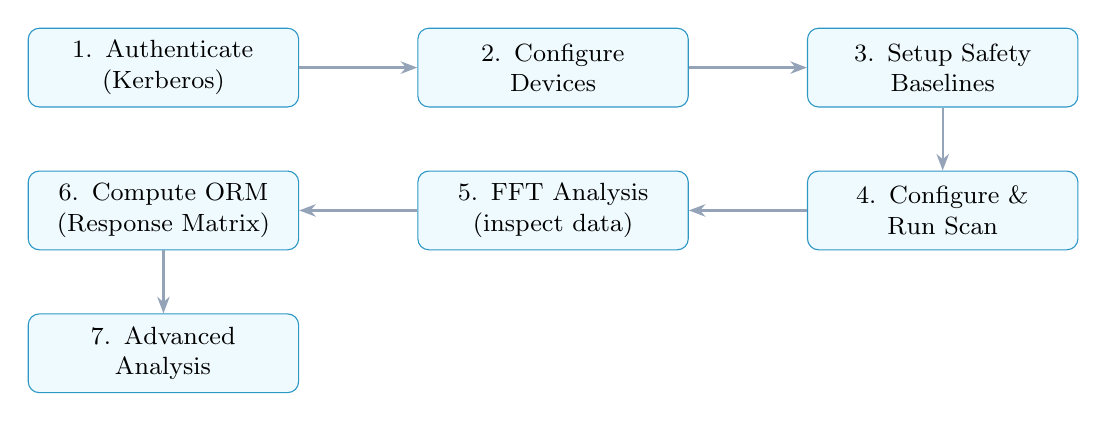
\begin{tikzpicture}[
  node distance=0.8cm and 1.5cm,
  block/.style={
    rectangle, rounded corners=4pt, draw=accent!80!black,
    fill=accent!8, text width=3.2cm, minimum height=1cm,
    align=center, font=\small
  },
  decision/.style={
    diamond, draw=warncol!80!black, fill=warncol!8,
    text width=2cm, align=center, aspect=2, font=\small
  },
  arrow/.style={-{Stealth[length=6pt]}, thick, color=mutedtext},
]
  \node[block] (auth)    {1. Authenticate\\(Kerberos)};
  \node[block, right=of auth] (devices) {2. Configure\\Devices};
  \node[block, right=of devices] (safety)  {3. Setup Safety\\Baselines};
  \node[block, below=of safety] (scan)    {4. Configure \&\\Run Scan};
  \node[block, left=of scan] (fft)     {5. FFT Analysis\\(inspect data)};
  \node[block, left=of fft] (orm)     {6. Compute ORM\\(Response Matrix)};
  \node[block, below=of orm] (analysis){7. Advanced\\Analysis};

  \draw[arrow] (auth)    -- (devices);
  \draw[arrow] (devices) -- (safety);
  \draw[arrow] (safety)  -- (scan);
  \draw[arrow] (scan)    -- (fft);
  \draw[arrow] (fft)     -- (orm);
  \draw[arrow] (orm)     -- (analysis);
\end{tikzpicture}
\caption{Typical \forma{} workflow.}\label{fig:workflow}
\end{figure}


% ═════════════════════════════════════════════════════════════════════════════
\chapter{Tab-by-Tab Reference}\label{ch:tabs}
% ═════════════════════════════════════════════════════════════════════════════

% ─────────────────────────────────────────────────────────────────────────────
\section{Tab 1: Device Settings \& Selection}\label{sec:tab1}

This tab is the starting point for every session.

\subsection{Authentication}

\begin{stepbox}[Step: Log in to Kerberos]
Click \btn{Kerberos Login} (or use \menupath{Authentication > Kerberos Login}).
Enter your Kerberos principal and password in the dialog. On success the status changes to \textcolor{accent2}{\textbf{Authenticated}} (green).
\end{stepbox}

\begin{warnbox}[Authentication Required]
Most hardware-interacting features (fetching nominals, applying settings, running scans) require valid Kerberos credentials. Always authenticate first.
\end{warnbox}

\subsection{Adding Devices}

There are two methods:

\subsubsection{Manual Entry}
\begin{enumerate}
  \item Type a device name in the \field{Device Name} field (e.g.\ \texttt{H:CORR01}).
  \item Click \btn{Add to Setting List} (for correctors) or \btn{Add to Reading List} (for BPMs).
  \item Repeat for each device.
\end{enumerate}

\subsubsection{File-Based Selection}
\begin{enumerate}
  \item Click \btn{Open Device Selection Tool\ldots}
  \item Select an Excel (\texttt{.xlsx}/\texttt{.xls}) or CSV file containing device names in the first column.
  \item A dialog shows the available sheets; select the ones to import.
  \item Devices are added to the appropriate list.
\end{enumerate}

The status labels at the bottom show the current count: e.g.\ ``\textit{12 devices in Setting List.}''

\subsection{Device Settings Grid}

After adding setting devices, a scrollable grid appears showing each device with an editable \field{New Value} field. This lets you set custom setpoints before a scan if needed.

\subsection{Control Buttons}

\begin{tabularx}{\textwidth}{lX}
  \toprule
  \textbf{Button} & \textbf{Action} \\
  \midrule
  \btn{Fetch Nominals}   & Reads the current operational values of all setting devices from \acnet{}. \\
  \btn{Apply Settings}    & Writes the values in the \field{New Value} fields to hardware (with confirmation dialog). \\
  \field{ACNET Role}      & Dropdown to select the control role: \texttt{OPERATOR}, \texttt{testing}, \texttt{linac\_trims}, \texttt{linac\_quads}. \\
  \btn{Clear Setting List} / \btn{Clear Reading List} & Removes all devices from the respective list. \\
  \bottomrule
\end{tabularx}

% ─────────────────────────────────────────────────────────────────────────────
\section{Tab 2: Scan Settings}\label{sec:tab2}

This tab configures scan parameters and launches the measurement.

\subsection{Global Parameters}

\begin{tabularx}{\textwidth}{lp{2cm}X}
  \toprule
  \textbf{Parameter} & \textbf{Default} & \textbf{Description} \\
  \midrule
  Points per Superperiod & 100 & Number of sample steps in one modulation cycle. More points give finer frequency resolution in the FFT. \\
  Number of Superperiods & 1   & How many complete cycles to execute. More cycles reduce noise by $\sqrt{N_{\text{sp}}}$. \\
  \bottomrule
\end{tabularx}

\subsection{Scan Mode}

\begin{tabularx}{\textwidth}{lX}
  \toprule
  \textbf{Mode} & \textbf{Description} \\
  \midrule
  \textbf{Simultaneous} (default) & All correctors modulate in parallel. Fastest option ($N\times$ speed-up). Each corrector should use a \emph{different} number of periods to separate their frequencies. \\
  \textbf{Sequential} & One corrector at a time. Maximum isolation and SNR but $N\times$ slower. \\
  \bottomrule
\end{tabularx}

\subsection{Per-Device Settings}

The treeview table shows one row per setting device with editable columns:

\begin{tabularx}{\textwidth}{lX}
  \toprule
  \textbf{Column} & \textbf{Meaning} \\
  \midrule
  \field{Device}            & Device name (read-only). \\
  \field{Amplitude}         & Peak amplitude of sinusoidal excitation (in device units). \\
  \field{Number of Periods} & How many full sine cycles within one superperiod. In simultaneous mode, each device \emph{must} have a unique value. \\
  \bottomrule
\end{tabularx}

Double-click any cell in the Amplitude or Number of Periods columns to edit it.

\subsection{Save Location}

Click \btn{Browse\ldots} to choose where scan data files will be saved. Default: current working directory.

\subsection{Scan Controls}

\begin{tabularx}{\textwidth}{lX}
  \toprule
  \textbf{Button} & \textbf{Action} \\
  \midrule
  \btn{Start Scan}       & Begins the measurement (button disables; Stop Scan enables). \\
  \btn{Stop Scan}        & Gracefully stops an in-progress scan and restores nominals. \\
  \btn{Preview Waveform} & Opens a popup window showing the computed sinusoidal waveforms for all devices. \\
  \btn{Save Scan Setup}  & Saves all scan parameters to a \texttt{.json} file. \\
  \btn{Load Scan Setup}  & Restores parameters from a previously saved \texttt{.json} file. \\
  \bottomrule
\end{tabularx}

\subsection{What Happens During a Scan}

\begin{enumerate}
  \item \forma{} fetches the nominal (current operational) values for all setting devices.
  \item For each step $n = 0, 1, \ldots, N_{\text{total}}{-}1$:
    \begin{enumerate}[label=(\alph*)]
      \item Computes the excitation value for each corrector using Eq.~\ref{eq:waveform}.
      \item Applies the settings to hardware via \acnet{}.
      \item Waits for the next \acnet{} event trigger, then reads all device readbacks.
      \item Stores the timestamp and readback values.
      \item Checks safety thresholds (if enabled).
    \end{enumerate}
  \item Progress bar advances with each step.
  \item On completion (or abort): restores all correctors to nominal values.
  \item Data is auto-saved to CSV with an accompanying \texttt{\_meta.json} file.
\end{enumerate}

\begin{dangerbox}[Safety Abort]
If the safety system detects an orbit deviation exceeding the abort threshold, the scan halts immediately, nominals are restored, and a detailed abort log is saved. See Section~\ref{sec:tab3} for configuration.
\end{dangerbox}

% ─────────────────────────────────────────────────────────────────────────────
\section{Tab 3: Safety Configuration}\label{sec:tab3}

The safety system provides real-time protection during scans.

\subsection{Safety Status Banner}

The banner at the top of this tab shows one of three states:

\begin{tabularx}{\textwidth}{llX}
  \toprule
  \textbf{State} & \textbf{Colour} & \textbf{Meaning} \\
  \midrule
  \textbf{DISABLED}       & \textcolor{mutedtext}{Grey}    & Safety monitoring is turned off. \\
  \textbf{NOT CONFIGURED} & \textcolor{warncol}{Yellow}    & Enabled but no baselines measured yet. \\
  \textbf{ACTIVE}         & \textcolor{accent2}{Green}     & Fully operational with $N$ devices monitored. \\
  \bottomrule
\end{tabularx}

\subsection{Setup Procedure}

\begin{stepbox}[Step 1: Enable Safety]
Check the box: ``\textit{Enable Safety Monitoring (stops scan if thresholds exceeded)}''.
\end{stepbox}

\begin{stepbox}[Step 2: Measure Baseline]
\begin{enumerate}
  \item Set \field{Number of Samples} (minimum~10, recommend~50--100).
  \item Click \btn{Measure Safety Baseline}.
  \item Wait for data collection to complete. The baseline table populates with: Device, Mean, RMS, Std Dev, Min, Max, Samples.
\end{enumerate}
\end{stepbox}

\begin{warnbox}[Important]
Measure baselines with \emph{no active excitation}. The baseline captures the natural noise floor; any deliberate orbit modulation will inflate the standard deviation and desensitise the safety system.
\end{warnbox}

\begin{stepbox}[Step 3: Configure Thresholds]
\begin{enumerate}
  \item \textbf{Monitoring Mode}: choose between:
    \begin{itemize}
      \item \textbf{Per-Device Mean} --- each BPM checked individually.
      \item \textbf{Overall Mean} --- combined mean across all BPMs.
    \end{itemize}
  \item \textbf{Averaging Window}: number of recent readings to average before checking (1 = no averaging).
  \item \textbf{Warning Threshold ($\sigma$)}: triggers a log message. Scan continues.
  \item \textbf{Abort Threshold ($\sigma$)}: halts the scan immediately.
  \item Click \btn{Apply Threshold Settings}.
\end{enumerate}
\end{stepbox}

\subsection{Save / Load / Clear}

\begin{tabularx}{\textwidth}{lX}
  \toprule
  \btn{Save Safety Config}    & Exports all baselines and thresholds to a \texttt{.json} file. \\
  \btn{Load Safety Config}    & Restores a previously saved configuration. \\
  \btn{Clear All Baselines}   & Deletes all baseline data (requires confirmation). \\
  \bottomrule
\end{tabularx}

% ─────────────────────────────────────────────────────────────────────────────
\section{Tab 4: Baseline RMS}\label{sec:tab4}

A standalone tool for measuring BPM noise floors, independent of the safety system.

\begin{enumerate}
  \item Set \field{Number of Samples} (default: 50).
  \item Click \btn{Measure Baseline RMS}.
  \item Results appear in the table: Device, RMS Fluctuation.
  \item Click \btn{Save RMS Data to CSV} to export.
\end{enumerate}

This is useful for characterising machine noise before deciding on scan amplitudes.

% ─────────────────────────────────────────────────────────────────────────────
\section{Tab 5: Data Reading and Plots}\label{sec:tab5}

Provides continuous live monitoring of device readbacks.

\subsection{Controls}

\begin{tabularx}{\textwidth}{lX}
  \toprule
  \btn{Start Reading} / \btn{Stop Reading} & Toggles continuous data acquisition. \\
  \btn{Save Live Data}   & Saves all accumulated data to CSV. \\
  \field{Device to Plot}  & Dropdown selecting which device's time series to display. \\
  \field{ACNET Event}     & Trigger event for data acquisition. Options: \texttt{@p,1000} (periodic 1\,s), \texttt{@i} (injection), \texttt{@e,52} (custom event). \\
  \bottomrule
\end{tabularx}

\subsection{Live Plot}

The plot shows the most recent 2000 data points for the selected device. The X-axis is timestamp, Y-axis is the readback value. The plot updates in real time during acquisition.

% ─────────────────────────────────────────────────────────────────────────────
\section{Tab 6: Statistics}\label{sec:tab6}

Displays summary statistics for all reading devices during live data acquisition.

\begin{tabularx}{\textwidth}{lX}
  \toprule
  \textbf{Column} & \textbf{Description} \\
  \midrule
  \field{Device}  & Device name. \\
  \field{Min}     & Minimum observed value. \\
  \field{Max}     & Maximum observed value. \\
  \field{Mean}    & Average value. \\
  \field{Std Dev} & Standard deviation. \\
  \bottomrule
\end{tabularx}

A summary label shows the \textbf{Overall RMS of Std Deviations} across all devices. Click \btn{Export to CSV} to save.

% ─────────────────────────────────────────────────────────────────────────────
\section{Tab 7: FFT Analysis}\label{sec:tab7}

An interactive spectral analysis tool for inspecting scan data.

\subsection{Loading Data}

Click \btn{Load Scan Data File} and select a scan CSV. The device listbox populates with all columns from the file. If a corresponding \texttt{\_meta.json} exists, scan parameters are loaded automatically.

\subsection{Generating FFT Plots}

\begin{enumerate}
  \item Select one or more devices in the listbox (Ctrl+Click for multiple).
  \item Click \btn{Generate FFT Plot}.
  \item The plot shows each device's amplitude spectrum.
\end{enumerate}

\subsection{Plot Features}

\begin{itemize}
  \item \textbf{X-axis}: Number of Periods (= number of complete cycles within the scan window).
  \item \textbf{Y-axis}: Normalised Amplitude.
  \item \textbf{Hover}: Moving the mouse over a peak shows an annotation with the exact period count and amplitude.
  \item \textbf{Colour coding}: Each device gets a distinct colour from the palette (cyan, orange, green, yellow, purple, pink).
\end{itemize}

\begin{notebox}[Verifying Scan Quality]
Use the FFT tab to check that:
\begin{itemize}
  \item Each corrector shows a clear peak at its configured number of periods.
  \item BPMs show peaks at the corrector frequencies (confirming response).
  \item The noise floor is well below the signal peaks (good SNR).
\end{itemize}
\end{notebox}

% ─────────────────────────────────────────────────────────────────────────────
\section{Tab 8: Response Matrix}\label{sec:tab8}

This is the primary output tab where the ORM is computed and visualised.

\subsection{Controls}

\begin{tabularx}{\textwidth}{lX}
  \toprule
  \btn{Calculate Response Matrix}  & Runs the full ORM computation (Section~\ref{sec:transfer}--\ref{sec:error}). Requires scan data to be loaded in the FFT tab. \\
  \btn{Save Matrix to CSV}          & Exports the matrix to separate CSV files per plane (horizontal/vertical) with corresponding error matrices. \\
  \btn{Open Advanced Analysis}       & Launches the PyQt5 analysis viewer (Chapter~\ref{ch:analysis}). \\
  \field{Auto-calculate ORM}         & Checkbox. If enabled, ORM is computed automatically after each scan completes. \\
  \bottomrule
\end{tabularx}

\subsection{Display Modes}

The \field{Display} dropdown switches between three visualisation modes:

\begin{tabularx}{\textwidth}{lX}
  \toprule
  \textbf{Mode} & \textbf{Description} \\
  \midrule
  \textbf{Gain (Real)}            & The response matrix $R_{ij}$ (Eq.~\ref{eq:Rij}). Blue/red coolwarm colourmap; sign indicates kick direction. \\
  \textbf{Uncertainty ($\sigma$)} & The error matrix $\Delta R_{ij}$ (Eq.~\ref{eq:errorprop}). Magma colourmap; brighter = larger uncertainty. \\
  \textbf{Device Noise}           & Noise floor characteristics. \\
  \bottomrule
\end{tabularx}

\subsection{Heatmap Display}

The tab shows two side-by-side heatmaps:
\begin{itemize}
  \item \textbf{Left}: Horizontal BPMs (names containing \texttt{BPH}).
  \item \textbf{Right}: Vertical BPMs (names containing \texttt{BPV}).
\end{itemize}
Each has its own colourbar. The X-axis labels are correctors; Y-axis labels are BPMs.

\subsection{Saved File Format}

When saving, \forma{} creates up to four files:
\begin{itemize}
  \item \texttt{response\_matrix\_<timestamp>\_horizontal.csv}
  \item \texttt{response\_matrix\_<timestamp>\_vertical.csv}
  \item \texttt{response\_matrix\_<timestamp>\_horizontal\_error.csv}
  \item \texttt{response\_matrix\_<timestamp>\_vertical\_error.csv}
\end{itemize}

Each CSV has BPM names as row indices and corrector names as column headers.

% ─────────────────────────────────────────────────────────────────────────────
\section{Tab 9: Activity Log}\label{sec:tab9}

All application messages are displayed here in a scrollable, colour-coded log:

\begin{tabularx}{\textwidth}{lll}
  \toprule
  \textbf{Prefix} & \textbf{Colour} & \textbf{Meaning} \\
  \midrule
  \texttt{[SUCCESS]} & \textcolor{accent2}{Green}    & Operation completed successfully. \\
  \texttt{[WARNING]} & \textcolor{warncol}{Orange}   & Non-critical issue; action may be needed. \\
  \texttt{[ERROR]}   & \textcolor{dangercol}{Red}    & Critical failure; check and resolve. \\
  \texttt{[INFO]}    & Grey                           & Informational message. \\
  \bottomrule
\end{tabularx}

Click \btn{Clear Log} to erase the log contents.


% ═════════════════════════════════════════════════════════════════════════════
\chapter{Advanced Analysis Viewer}\label{ch:analysis}
% ═════════════════════════════════════════════════════════════════════════════

The analysis viewer is a separate PyQt5 application that provides interactive exploration of the response matrix.

\section{Launching}

There are three ways to open the viewer:

\begin{enumerate}
  \item \textbf{From \forma{}}: Click \btn{Open Advanced Analysis} in the Response Matrix tab. Data is passed in-memory.
  \item \textbf{From command line}:
    \begin{lstlisting}[language=bash]
python analysis_viewer.py --file response_matrix.csv
    \end{lstlisting}
  \item \textbf{Programmatically}:
    \begin{lstlisting}[language=Python]
from analysis_viewer import launch_from_arrays
proc = launch_from_arrays(matrix, row_labels, col_labels,
                          error_matrix, plane_map)
    \end{lstlisting}
\end{enumerate}

\section{Window Layout}

The viewer has a dark theme matching \forma{}. The layout is:

\begin{figure}[H]
\centering
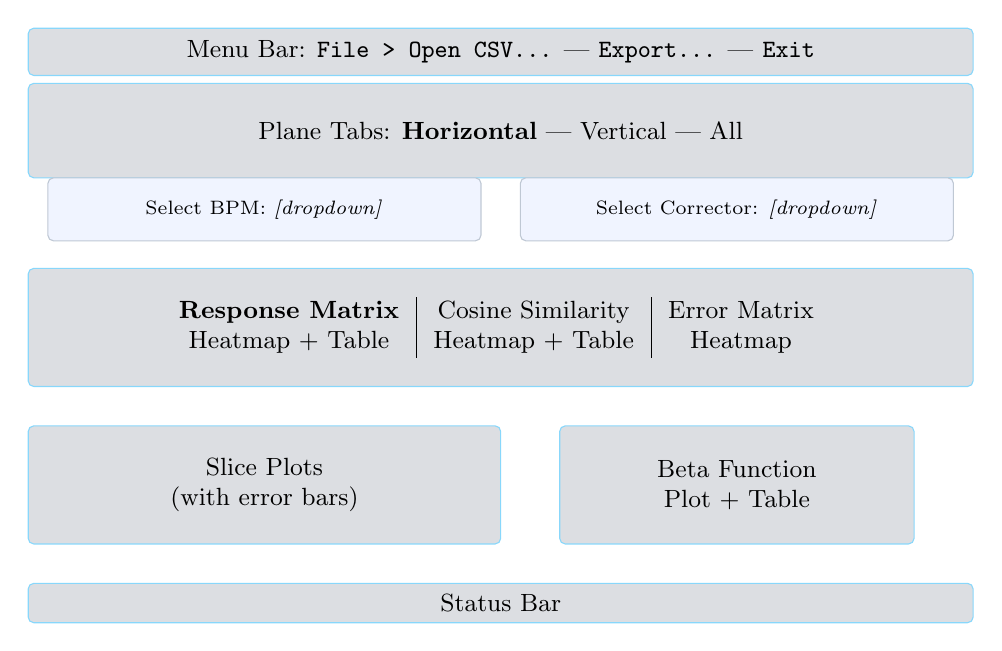
\begin{tikzpicture}[
  box/.style={rectangle, draw=accent!60, fill=card!15,
    minimum width=4cm, minimum height=1.2cm, align=center, font=\small,
    rounded corners=2pt},
  smallbox/.style={rectangle, draw=mutedtext!60, fill=lightbg,
    minimum width=3cm, minimum height=0.8cm, align=center, font=\scriptsize,
    rounded corners=2pt},
]
  % Menu
  \node[box, minimum width=12cm, minimum height=0.6cm] (menu)
    at (0,5) {Menu Bar: \menupath{File > Open CSV\ldots} | \menupath{Export\ldots} | \menupath{Exit}};

  % Plane tabs
  \node[box, minimum width=12cm] (planetabs)
    at (0,4) {Plane Tabs: \textbf{Horizontal} | Vertical | All};

  % Selectors
  \node[smallbox, minimum width=5.5cm] (bpm) at (-3,3) {Select BPM: \field{[dropdown]}};
  \node[smallbox, minimum width=5.5cm] (corr) at (3,3) {Select Corrector: \field{[dropdown]}};

  % Secondary tabs
  \node[box, minimum width=12cm, minimum height=1.5cm] (sectabs)
    at (0,1.5) {%
      \begin{tabular}{c|c|c}
        \textbf{Response Matrix} & Cosine Similarity & Error Matrix \\
        Heatmap + Table & Heatmap + Table & Heatmap
      \end{tabular}
    };

  % Lower
  \node[box, minimum width=6cm, minimum height=1.5cm] (slices)
    at (-3,-0.5) {Slice Plots\\(with error bars)};
  \node[box, minimum width=4.5cm, minimum height=1.5cm] (beta)
    at (3,-0.5) {Beta Function\\Plot + Table};

  % Status
  \node[box, minimum width=12cm, minimum height=0.5cm] (status)
    at (0,-2) {Status Bar};
\end{tikzpicture}
\caption{Analysis viewer layout.}\label{fig:viewer-layout}
\end{figure}

\section{Plane Tabs}

If a plane map is provided (e.g.\ from \forma{}), separate tabs are created for each plane:
\begin{itemize}
  \item \textbf{Horizontal} --- only BPMs containing \texttt{BPH} in their name.
  \item \textbf{Vertical} --- only BPMs containing \texttt{BPV} in their name.
  \item \textbf{All} --- full matrix (added if not all rows are covered by the plane map).
\end{itemize}

Each plane tab is fully independent with its own selectors, plots, and tables.

\section{Response Matrix Sub-Tab}

\begin{itemize}
  \item \textbf{Left panel}: Heatmap coloured with the \texttt{viridis} colourmap. Axes show BPM names (rows) and corrector names (columns).
  \item \textbf{Right panel}: Numerical table showing the matrix values to 4~decimal places. Entries that were not computed show ``N/A''.
\end{itemize}

\section{Cosine Similarity Sub-Tab}

Shows the corrector-to-corrector similarity matrix (Eq.~\ref{eq:cossim}):
\begin{itemize}
  \item \textbf{Heatmap}: Square matrix with corrector labels on both axes. Diagonal is always~1.0.
  \item \textbf{Table}: Numerical values to 4~decimal places.
\end{itemize}

\begin{notebox}[Identifying Redundant Correctors]
Corrector pairs with $S_{kl}\approx1$ have nearly identical effects on the orbit. One of them may be redundant for correction purposes.
\end{notebox}

\section{Error Matrix Sub-Tab}

Displays the uncertainty matrix $\Delta R_{ij}$ (Eq.~\ref{eq:errorprop}) as a heatmap with the \texttt{magma} colourmap (dark~=~low uncertainty, bright~=~high). This tab is only enabled if error data was provided.

\section{Slice Plots}

The lower-left panel shows two interactive plots that update when you change the BPM or corrector selection in the dropdowns:

\begin{itemize}
  \item \textbf{Top plot} --- \textcolor{accent}{\textbf{BPM Response}}: for the selected BPM, shows $R_{i,\bullet}$ (response to every corrector). Plotted as cyan circles connected by lines, with error bars (lavender caps) if available.
  \item \textbf{Bottom plot} --- \textcolor{accent2}{\textbf{Corrector Response}}: for the selected corrector, shows $R_{\bullet,j}$ (response at every BPM). Plotted as green squares with error bars.
\end{itemize}

\begin{notebox}[Reading the Error Bars]
The error bars represent $\pm\Delta R_{ij}$ from Eq.~\ref{eq:errorprop}. A BPM--corrector pair with a large error bar relative to the response value has low measurement confidence and may benefit from:
\begin{itemize}
  \item Larger corrector excitation amplitude,
  \item More scan points (better frequency resolution),
  \item More superperiods (noise averaging).
\end{itemize}
\end{notebox}

\section{Beta Function}

The lower-right panel shows the estimated betatron function (Section~\ref{sec:svd}):

\begin{itemize}
  \item \textbf{Plot}: $\hat{\beta}_i$ vs.\ BPM index, plotted as orange circles.
  \item \textbf{Table}: Two columns --- BPM name and $\hat{\beta}$ value (6~decimal places), or ``N/A'' if not computable.
\end{itemize}

\section{File Menu}

\begin{tabularx}{\textwidth}{lX}
  \toprule
  \menupath{File > Open Response CSV\ldots} & Load a response matrix from a CSV file. First column is the row index (BPM names), header row has corrector names. \\
  \menupath{File > Export Current Plane\ldots} & Save the current plane's matrix to a new CSV file. \\
  \menupath{File > Exit} & Close the viewer. \\
  \bottomrule
\end{tabularx}


% ═════════════════════════════════════════════════════════════════════════════
\chapter{Data Files and Formats}\label{ch:data}
% ═════════════════════════════════════════════════════════════════════════════

\section{Scan Data CSV}

\begin{lstlisting}
Timestamp, H:CORR01, H:CORR02, BPH:01, BPH:02, ...
2025-01-15 10:30:45.123, 0.50, -0.32, 1.234, 0.567, ...
2025-01-15 10:30:46.135, 0.53, -0.30, 1.245, 0.578, ...
...
\end{lstlisting}

\begin{itemize}
  \item First column: ISO-format timestamps.
  \item Remaining columns: readback values for each device (both correctors and BPMs).
  \item Correctors use actual readback values, not commanded setpoints.
\end{itemize}

\section{Scan Metadata JSON}

\begin{lstlisting}
[
  {"device": "H:CORR01", "amplitude": 0.5, "periods": 2},
  {"device": "H:CORR02", "amplitude": 0.3, "periods": 3}
]
\end{lstlisting}

One entry per corrector. Saved alongside the scan CSV with suffix \texttt{\_meta.json}.

\section{Response Matrix CSV}

\begin{lstlisting}
Reading Device, H:CORR01, H:CORR02, ...
BPH:01, 0.4532, 0.1234, ...
BPH:02, 0.3812, -0.0567, ...
\end{lstlisting}

Row index: BPM names. Columns: corrector names. Values: $R_{ij}$. Missing entries appear as empty cells (NaN).

\section{Error Matrix CSV}

Same format as the response matrix CSV but with $\Delta R_{ij}$ values. Saved with suffix \texttt{\_error.csv}.

\section{Safety Configuration JSON}

Contains: enabled flag, threshold type, per-device and overall warning/abort thresholds, buffer size, and all device baselines (mean, RMS, std, min, max, sample count).

\section{Scan Setup JSON}

Contains: points per superperiod, number of superperiods, scan mode, per-device amplitudes and period counts.


% ═════════════════════════════════════════════════════════════════════════════
\chapter{Tips and Best Practices}\label{ch:tips}
% ═════════════════════════════════════════════════════════════════════════════

\section{Choosing Scan Parameters}

\begin{defbox}[Parameter Selection Guidelines]
\begin{itemize}
  \item \textbf{Amplitude}: Large enough for clear signal above BPM noise. Use the Baseline RMS tab (Tab~4) to gauge the noise floor. A rule of thumb: amplitude should produce orbit changes at least 5$\times$ the BPM RMS noise.
  \item \textbf{Points per superperiod}: At least $4\times$ the highest number of periods (Nyquist). Recommend 50--200.
  \item \textbf{Number of periods}: In simultaneous mode, assign a \emph{unique} value to each corrector. Avoid integer multiples (e.g.\ 2 and 4) to prevent harmonic overlap. Good choices: consecutive primes or well-separated integers.
  \item \textbf{Number of superperiods}: More superperiods improve SNR. Use 1--3 for quick checks, 5+ for production measurements.
\end{itemize}
\end{defbox}

\section{Simultaneous vs.\ Sequential}

\begin{tabularx}{\textwidth}{lXX}
  \toprule
  & \textbf{Simultaneous} & \textbf{Sequential} \\
  \midrule
  Speed        & Fast ($1\times$)            & Slow ($N\times$)            \\
  SNR          & Lower (shared bandwidth)     & Higher (isolated signal)    \\
  Cross-talk   & Possible (harmonic overlap)  & None                        \\
  Best for     & Routine measurements         & Precision measurements      \\
  \bottomrule
\end{tabularx}

\section{Interpreting the Response Matrix}

\begin{itemize}
  \item \textbf{Large positive/negative $R_{ij}$}: Strong coupling between corrector~$j$ and BPM~$i$. Sign indicates direction.
  \item \textbf{Near-zero $R_{ij}$ with small error bar}: Genuine weak coupling (BPM is near a node of the betatron oscillation).
  \item \textbf{Near-zero $R_{ij}$ with large error bar}: Inconclusive --- measurement noise dominates. Consider increasing the scan amplitude or number of superperiods.
  \item \textbf{NaN entries}: Pair was not computed (e.g.\ missing data or failed FFT). These are displayed as blank cells and transparent pixels in heatmaps.
\end{itemize}

\section{Interpreting Error Bars}

\begin{itemize}
  \item Error bars represent $\pm1\sigma$ uncertainty from Eq.~\ref{eq:errorprop}.
  \item If error bars are much larger than the response value, the measurement is noise-dominated.
  \item To reduce error bars: increase corrector amplitude ($A_c$), add more scan points, or add more superperiods.
  \item The two dominant contributions are:
    \begin{enumerate}
      \item BPM noise ($\sigma_b$): reduced by stronger excitation.
      \item Corrector noise ($\sigma_c$): reduced by cleaner power supplies or longer averaging.
    \end{enumerate}
\end{itemize}

\section{Safety System Recommendations}

\begin{warnbox}[Safety Best Practices]
\begin{itemize}
  \item Always measure baselines \emph{without} any active excitation.
  \item Set the warning threshold at $3\sigma$ and abort at $5\sigma$ as starting values.
  \item Use the averaging window (buffer size) to smooth transient spikes: 5--20 samples is typical.
  \item After loading a safety configuration, verify that baselines are still valid for current machine conditions.
  \item Review abort logs after any safety event to understand what happened.
\end{itemize}
\end{warnbox}


% ═════════════════════════════════════════════════════════════════════════════
\appendix
\chapter{Quick Reference Card}\label{app:quickref}
% ═════════════════════════════════════════════════════════════════════════════

\begin{center}
\small
\begin{tabularx}{0.95\textwidth}{>{\raggedright\arraybackslash}p{3.5cm}X}
  \toprule
  \textbf{Action} & \textbf{How} \\
  \midrule
  Authenticate         & Tab~1 $\to$ \btn{Kerberos Login} \\
  Add devices          & Tab~1 $\to$ Manual entry or \btn{Open Device Selection Tool\ldots} \\
  Preview waveform     & Tab~2 $\to$ \btn{Preview Waveform} \\
  Run scan             & Tab~2 $\to$ \btn{Start Scan} \\
  Stop scan            & Tab~2 $\to$ \btn{Stop Scan} \\
  Setup safety         & Tab~3 $\to$ Enable $\to$ Measure Baseline $\to$ Set Thresholds \\
  Measure BPM noise    & Tab~4 $\to$ \btn{Measure Baseline RMS} \\
  Live monitoring      & Tab~5 $\to$ \btn{Start Reading} \\
  Inspect FFT          & Tab~7 $\to$ \btn{Load Scan Data File} $\to$ Select devices $\to$ \btn{Generate FFT Plot} \\
  Compute ORM          & Tab~8 $\to$ \btn{Calculate Response Matrix} \\
  View with errors     & Tab~8 $\to$ \btn{Open Advanced Analysis} \\
  Save ORM             & Tab~8 $\to$ \btn{Save Matrix to CSV} \\
  Auto-compute ORM     & Tab~8 $\to$ Check ``Auto-calculate ORM after scan'' \\
  \bottomrule
\end{tabularx}
\end{center}

% ═════════════════════════════════════════════════════════════════════════════
\chapter{Key Equations Summary}\label{app:equations}
% ═════════════════════════════════════════════════════════════════════════════

\begin{align}
  \text{DFT:}\quad
  & X[k] = \textstyle\sum_{n=0}^{N-1} x[n]\,e^{-j2\pi kn/N}
    \tag{\ref{eq:dft}} \\[8pt]
  \text{Amplitude:}\quad
  & A[k] = \tfrac{2}{N}\,|X[k]|
    \tag{\ref{eq:amp}} \\[8pt]
  \text{Transfer function:}\quad
  & R_{ij} = \operatorname{Re}\!\bigl(\tilde{A}_{b,i}/\tilde{A}_{c,j}\bigr)
    \tag{\ref{eq:Rij}} \\[8pt]
  \text{Error:}\quad
  & \Delta R_{ij} = \sqrt{
      \frac{\sigma_b^2}{2A_c^2}
      + \frac{A_b^2\,\sigma_c^2}{2A_c^4}
    }
    \tag{\ref{eq:errorprop}} \\[8pt]
  \text{Beta function:}\quad
  & \hat{\beta}_i = (U_{i,1}\,\sigma_1)^2
    \tag{\ref{eq:beta}} \\[8pt]
  \text{Cosine similarity:}\quad
  & S_{kl} = \hat{\mathbf{c}}_k\cdot\hat{\mathbf{c}}_l
    \tag{\ref{eq:cossim}} \\[8pt]
  \text{Safety deviation:}\quad
  & n_{\sigma} = |\bar{x} - \mu^{(0)}|\,/\,\sigma^{(0)}
    \tag{\ref{eq:safetydev}}
\end{align}


% ═════════════════════════════════════════════════════════════════════════════
\end{document}
